\documentclass[12pt]{beamer}
\usetheme{Warsaw}
\usepackage[utf8]{inputenc}
\usepackage[german]{babel}
\usepackage[T1]{fontenc}
\usepackage{amsmath}
\usepackage{amsfonts}
\usepackage{amssymb}
\usepackage{graphicx}
\author{Veronica Schier, Adrian Löwenberg Casas, \\Julien Caselmann}
\title{Die Kuen'sche Fläche}
%\setbeamercovered{transparent} 
%\setbeamertemplate{navigation symbols}{} 
%\logo{} 
%\institute{} 
%\date{} 
%\subject{} 
\begin{document}

\begin{frame}
\titlepage
\end{frame}

\begin{frame}

\tableofcontents

\end{frame}

\section{Geschichte}
\begin{frame}{Ursprung und Entdeckung}

\begin{itemize}
\item benannt nach Theodor Kuen 
\item experimentierte mit Bianchi-Transformationen und der Pseudosphäre
\item viel Vorarbeit in der Differentialgeometrie durch Luigi Bianchi \cite{bianchi_wiki}
\end{itemize}

\end{frame}

\begin{frame}

\begin{center}
\textit{\glqq Die schönste Bianchi - Transformation der Pseudosphäre\grqq}
\end{center}

\begin{tiny}
\begin{flushright}
\textit{- Jeder Mathematiker, immer\phantom{aaa}}
\end{flushright}
\end{tiny}

\end{frame}

\section{Zugrundeliegende Mathematik}
\begin{frame}
\begin{enumerate}
\item Pseudosphäre
\item Bianchi-Kongruenzen
\item Bianchi-Transformationen
\end{enumerate}
\end{frame}

\begin{frame}{Pseudosphäre}

\begin{itemize}
\item untersucht von Ferdinand Minding und Eugene Beltrami in 1868
\item Differentialgeometrie: Fläche mit konstanter, negativer Gaußkrümmung\cite{pseudo_wiki}
\item Pseudosphäre mit Radius $R$: Fläche mit konstanter, negativer Gaußkrümmung $-\frac{1}{R^2}$ \cite{pseudo_mathcurve}
 \cite{pseudo_wiki}
\end{itemize}

\end{frame}

\begin{frame}{Beispiele einer Pseudosphäre}

\begin{itemize}
\item Hyperboloid
\item Traktrikoid
\item theoretische Oberflächen
\end{itemize}

\end{frame}

\begin{frame}{Beispiel: Traktrikoid}

\begin{itemize}
\item Traktrix = Schleppkurve
\item Traktrikoid = Drehfläche einer Traktrix
\end{itemize}

\end{frame}

\begin{frame}{Beispiel: Traktrikoid}

\begin{center}
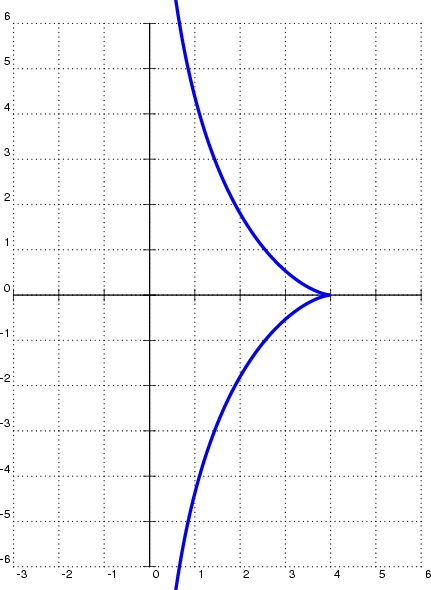
\includegraphics[scale=0.2]{traktrix.png}
\end{center}

\end{frame}

\begin{frame}{Beispiel: Traktrikoid}

\begin{center}
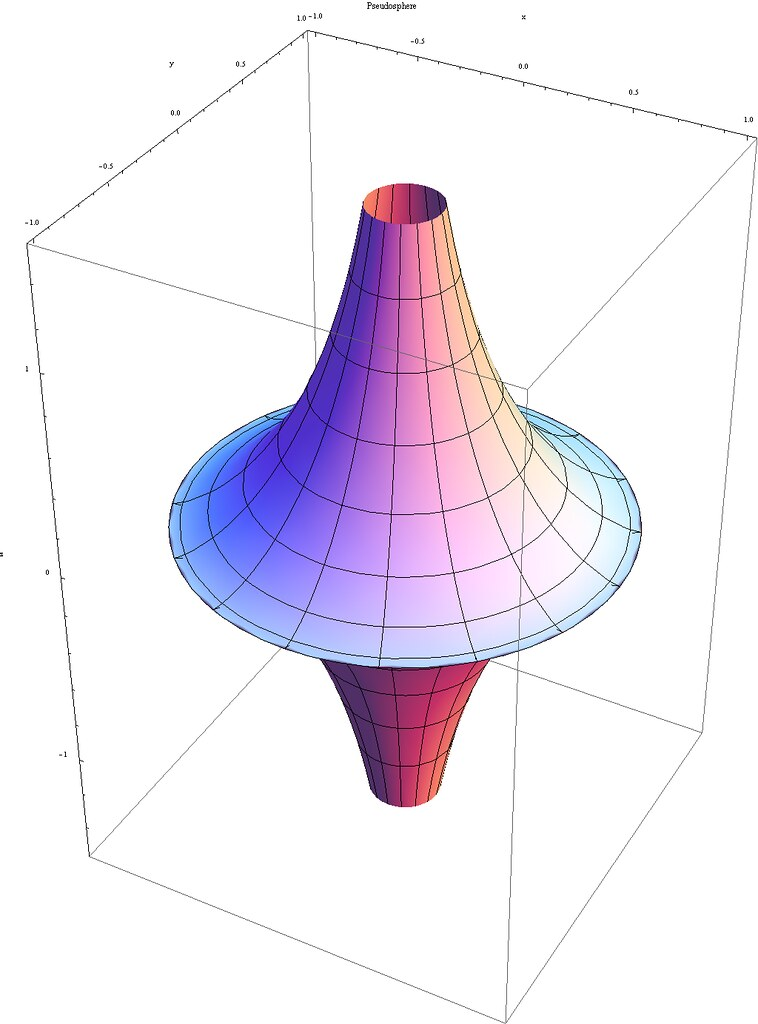
\includegraphics[scale=0.2]{pseudosphere.png}
\end{center}

\end{frame}

\begin{frame}{Bianchi - Kongruenzen}

\begin{itemize}
\item Kongruenz von Geraden
\item Krümmungen der Brennflächen an den Punkten einer Geraden sind alle gleich und negativ
\item Kongruenzgeraden bilden die asymptotischen Netze auf den Brennflächen auf ein orthogonales Netz auf einer Sphäre ab \cite{b_congruence_enc}
\end{itemize}

\end{frame}

\begin{frame}{Bianchi - Kongruenzen}
Krümmung einer Brennfläche einer Bianchi - Kongruenz:
\newline 
\begin{center}
$K = \frac{1}{(\phi(u) + \psi(v))^2}$
\end{center}


Jede Fläche, deren Krümmungen diese Bedingung erfüllen, ist eine Bianchi - Fläche \cite{b_congruence_enc}
\end{frame}

\begin{frame}{Bianchi - Transformationen}

\begin{itemize}
\item Übergang einer Brennfläche $S$ einer Bianchi - Kongruenz in die andere Brennfläche $S'$ derselben Bianchi - Kongruenz
\item $S$ Pseudosphäre $\Rightarrow S'$ Pseudosphäre
\item behält Gesamtkrümmung bei
\end{itemize}

\end{frame}


\section{Parametrisierung}
\begin{frame}{Parametrisierung der Kuen'schen Fläche}

\begin{center}
$
\begin{pmatrix}
x\\y\\z
\end{pmatrix}
 =
\begin{pmatrix}
\frac{2cosh(u)* \left( cos(v) + v*sin(v) \right)}{v^2+cosh(u)^2}\\\\
\frac{2cosh(u)*(sin(v) - v*cos(v))}{v^2 + cosh(u)^2}\\\\
\frac{sinh(2u)}{v^2 + cosh(u)^2}
\end{pmatrix}
u,v \in \left[ -2\pi , 2\pi \right] $
\end{center}

\end{frame}

\begin{frame}

\footnotesize{
\begin{thebibliography}{99}

\bibitem[Wiki] {pseudo_wiki} Wikipedia
\newblock Die Pseudosphäre
\newblock \emph{https://de.wikipedia.org/wiki/Pseudosph\%C3\%A4re}
\newblock 5. Dezember 2019

\bibitem[Mathcurve] {pseudo_mathcurve} Mathcurve
\newblock The pseudosphere
\newblock \emph{https://www.mathcurve.com/surfaces.gb/\\pseudosphere/pseudosphere.shtml}
\newblock 5. Dezember 2019

\bibitem[Wiki] {bianchi_wiki} Wikipedia
\newblock Luigi Bianchi
\newblock \emph{https://de.wikipedia.org/wiki/Luigi\_ Bianchi}
\newblock 12. Dezember 2019

\end{thebibliography}
}

\end{frame}

\begin{frame}

\footnotesize{
\begin{thebibliography}{99}

\bibitem[Encycl.] {b_congruence_enc} Encyclopedia of Mathematics
\newblock Bianchi congruence
\newblock \emph{https://www.encyclopediaofmath.org/index.php/Bianchi\_ congruence}
\newblock 12. Dezember 2019

\bibitem[Encycl.] {b_transform_enc} Encyclopedia of Mathematics
\newblock Bianchi transformation
\newblock \emph{https://www.encyclopediaofmath.org/index.php/Bianchi\_ transformation}
\newblock 12. Dezember 2019

\end{thebibliography}
}

\end{frame}


\end{document}